\chapter{Tribler, TrustChain and Implementation}
\label{chap:implementation}

Distributed trust systems rely heavily on the records of interactions. Our theoretical analysis from
the previous chapter has further shown that dissemination of those records is required to ensure the
validity of those records and therefore the trust that is built on them. In previous work our 
research group has created the tamper-proof recording system for interactions, TrustChain. This system is 
implemented in a peer-to-peer video streaming service Tribler and the IPv8 project\footnote{https://github.com/tribler/py-ipv8}.
% Although the exchange of information is part of those systems and as shown key to their manipulation
% resistance, exchanges are not explicitly recorded. 
With respect to our model though, TrustChain is limited in its ability to ensure gossiping because information
exchange is not recorded.
As such, the model of Chapter \ref{chap:model}
cannot be realized in their architecture. We created an extension of TrustChain that allows for the 
recording and reasoning about gossip behavior of agents.

We open this chapter by relating the previously introduced model to an application context. Next we
introduce the conceptual working of blockchains which is a core technology for TrustChain. A discussion of
TrustChain itself follows. Then our extension, the recording of exchanges, is discussed in detail. 
Finally, a more elaborate discussion of possible attacks on the system is performed.

\section{Relating Tribler to the ordered encounter model}
In the previous chapter the ordered encounter model was introduced which contains agents, interactions,
exchanges. The model is useful for studying the mechanisms of a trust system in a theoretical 
setting. However it may not be immediately obvious to the reader how the model relates to a digital
trust system in an application context. In this section we shed more light on how the concepts 
relate to their counterparts in the Tribler application.

We introduced Tribler in Chapter \ref{chap:introduction}. It is a peer-to-peer video streaming 
service which is based on the BitTorrent protocol. As the BitTorrent protocol does not guarantee the
privacy of users, Tribler adds an onion routing layer on top of the protocol. This routing protocol 
is similar to the Tor network and ensures that traffic is encrypted and relayed multiple times before exiting the
Tribler network and entering the public internet. The origin of the original request is made anonymous.

\subsection{Agents}
In the model, agents are the entities that take part in interactions and encounters. Intuitively one
would assume that users are the agents in Tribler. It would be more accurate though to see that a 
running instance of the Tribler software is the agent. A single human user can have multiple 
instances of the software running on multiple machines and thus ``control'' multiple agents. Despite
being able to run or stop the agents, the human user has only a very small decision space, though, 
because the software runs on its own and executes according to design. 

The distinction of honest and dishonest agents is then made as follows: honest agents are the 
instances that run the software as intended while dishonest agents are instances of manipulated 
software. 

Each running instance of the Tribler software can be uniquely identified. It makes use of asymmetric
cryptography for authentication and encryption. Specifically, Curve25519 is used in an 
elliptic curve Diffie-Hellman key agreement scheme. 

In the following description of the system we will use both, ``node'' and ``agent'' when referring to the 
behavior of a Tribler instance executing some action. 

\subsection{Interactions}
The interactions that we defined in the ordered interaction model map very well to the transactions
of data in Tribler. Peer-to-peer video streaming in Tribler works through uploading and downloading 
portions of data from any agent in the Tribler network based on the BitTorrent protocol. Also, as
mentioned above, agents relay traffic in the Tribler network for peers. Relaying again can be seen 
as a similar transaction where the incoming data is downloaded and immediately uploaded to the next
agent in the routing scheme. These transactions of data map to the transactions in our model and 
need to be recorded in a tamper-proof manner. For this recording of transaction Tribler implements 
TrustChain, which is discussed in 
more detail in Section~\ref{sec:trustchain}. The discussion of how to create those records, secure 
them against manipulations and distribute them in the network is the centerpiece of this work.

\subsection{Trust and reputation}
The uploading and downloading of videos in the network is a social dilemma as each user wants to 
stream videos while contributing as little as possible. It is therefore a good test bed for a trust 
system which records the behavior of users. The reputation of an agent in Tribler represents the 
contribution behavior of that agent. Contributing, that is uploading video streams to other users,
increases an agent's reputation whereas downloading, that is streaming videos, decreases an agent's 
reputation. Also, relaying is a neutral activity in terms of a upload-download ratio, yet the 
reputation of an agent that relays a lot of data needs to be higher as well. In contrast to 
reputation, trust is subjective and can be seen as the subjective notion of a peer being a 
``good contributor''. 

In order to better illustrate the difference between reputation and trust we provide an example.
Assume an agent $a$ knows two agents, $b$ and $c$ and sees that both have uploaded and downloaded 
the same amount of data. However, $b$ has $uploaded$ most to $a$ while $c$ has uploaded only to 
agents that $a$ has not heard of. Human intuition tells us that $a$ should trust $b$ more than $c$, 
because of the stronger direct connection. Trust therefore depends on the topography of the network.

% % 
% % Is this necessary??? 
% \section{Reciprocity}
% % 

\subsection{Exchanges}
As we have shown in Chapter \ref{chap:model}, the exchange of information is a major component of a trust 
systems defense against manipulators and free-riders. Yet, TrustChain does not create records on 
gossip. We identify this as a limitation. 

Honest Tribler agents actually do exchange data in order to calculate a non-zero reputation for possible
future peers. Still, without recording of this behavior, it cannot be rewarded or its absence be punished. 
This is why we propose an extended TrustChain which enables recording of gossip and gossip-about-gossip. 
The details of this extension are discussed in Section \ref{sec:extension}.

\section{Blockchain basics}
The design of distributed databases bears many challenges. Especially if sensitive data is involved
and users need to have access globally, the asynchrony of events, lack of guarantees on data 
consistency and agent honesty create issues. For the early years of the internet those challenges seemed
insurmountable. That is why most services that act on sensitive data are centralized, examples being 
banks, government institutions or commercial services like Facebook\footnote{https://facebook.com}.
Centralization has its own shortcomings such as abuse of power, dishonesty, single point-of-failure
and platform lock-in. We described those issues in more detail in Chapter \ref{chap:introduction}.
The increasing significance of those issues led to the design and implementation of the Bitcoin 
protocol~\cite{nakamoto2008bitcoin}. The Bitcoin protocol allows a distributed network of agents 
to agree on the exact order of events, through a hash chain which acts as a distributed timestamp 
server and the proof-of-work algorithm. This architecture is commonly referred to as Blockchain. We
shall introduce this concept in more detail as the core concepts are also applied in TrustChain.

\subsection{Concept}
A blockchain is essentially an append-only database in form of chained blocks. Each block on the 
chain contains a set of transactions, the root hash of that set, a unique identifier called the 
Nonce and the hash of the previous block. Through the hash of the previous block the blocks are 
chained together and a full sequence is created. Transactions and new blocks need to be published publicly on 
the network. Blocks may be created and published by any agent, but only after that agent guessed 
the solution to a probabilistic puzzle. This process is called mining but is not of importance to 
the discussion of this paper. Once selected, the agent adds transactions in the sequence as they 
were received. The block size is fixed such that after adding a certain number of 
transactions the block is considered complete. Once complete, the agent publishes the
block as well as the hash of the block's content. Any agent that receives the block will verify that
the solution to the puzzle is correct and all transactions are valid. If so, they add the new block
to their copy of the chain and start with solving the next puzzle in order to become the next selected
creator of a block.

\begin{figure}
    \centering
    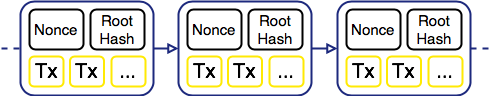
\includegraphics[width=0.7\textwidth]{images/blockchain}
    \caption{Conceptual depiction of a slice of a Bitcoin-like blockchain. Blocks contain multiple transactions and are chained together through the hash of the previous block. Source: \textit{Creation of TU Delft BLockchain Lab}}
    \label{fig:basic_blockchain}
\end{figure}

All agents are acting on the same copy of the blockchain. The one global chain therefore contains 
all transactions that happen on the network. This implies that all agents need to be informed about any new block.
In order to allow for enough time to synchronize transactions and blocks, the difficulty of the puzzle 
can be increased. This ensures a approximately fixed time between new blocks. This block time is 
10 minutes for Bitcoin. Together with the fixed block size the global transaction throughput of the
system is capped. For Bitcoin this is approximately 7 transactions per second.

\subsection{Tamper-proof}


\subsection{Incentive}


\section{TrustChain}
\label{sec:trustchain}

\subsection{Implementation details}

\section{Extension}
\label{sec:extension}


\subsection{Data}
\subsection{}
\subsection{Scalability concerns}

\section{Attacks}